\chapter{Lezione 1 - Approccio quantitativo al progetto e all'analisi. Parte 1}


In questo corso ci occuperemo dell'architettura dei sistemi di elaborazione, della loro descrizione sia interna che funzionale. Inizieremo questo ciclo di lezioni affrontando e descrivendo un approccio quantitativo al progetto e all'analisi. Questa lezione è costituita da due parti, oggi ci occuperemo della prima parte.
Ogni lezione sarà organizzata descrivendovi un sommario in cui affronteremo i problemi della lezione. Il primo argomento del sommario sono le tendenze nell'industria dei calcolatori. Successivamente discuteremo brevemente dell'era post PC


Argomenti trattati:
\begin{itemize}
    \item tendenze nell'industria dei calcolatori
    \item L'era Post-PC
\end{itemize}

Cominciamo con affrontare il primo degli argomenti, le tendenze nell'industria dei calcolatori.

\section{Tendenze nell'industria dei calcolatori}

Quando intendo dire tendenze, intendo dire l'evoluzione storica che sia avuta negli anni.

Durante la seconda guerra mondiale i calcolatori elettromeccanici ed elettronici per la decriptazione di codici furono sviluppati prevalentemente dai britannici e dagli americani per decriptare il cosiddetto Enigma, che era un sistema di decriptazione utilizzato per consentire le comunicazioni da e per i sottomarini tedeschi che affondavano ripetutamente le navi che transitavano attraverso l'Atlantico, trasportando materiali e uomini dagli Stati Uniti alla Gran Bretagna durante le prime fasi della guerra.

Questo è stato chiaramente un argomento di evidente rilevanza per il momento che ha portato le migliori menti a cimentarsi per la prima volta nell'utilizzo di macchine automatiche finalizzate a rompere questi codici, cioè a capire quali fossero le chiavi dei codici e quindi una volta identificate le chiavi poter decriptare i messaggi trasmessi. Ovviamente quando l'algoritmo fu decriptato non fu fatto scoprire ai tedeschi anche con non poco sacrificio delle proprie forze umane.
La cosa però è importante capire è che c'è stato un fortissimo motore che ha spinto lo sviluppo della tecnologia.
Notate che nella slide fig. \ref{fig:slide_4} è scritto esplicitamente calcolatori elettromeccanici ed elettronici.

\begin{figure}[ht]
    \centering
    \includegraphics[width=0.6\linewidth]{images/Lez01_P01_fig_04.png}
    \caption{Slide 4}
    \label{fig:slide_4}
\end{figure}

Con questo intendo dire che i calcolatori, per come la maggior parte di voi ormai è familiare, sono ben lontani da quello che erano agli albori dello sviluppo.
Il termine di elettromeccanici si intende che i selettori commutatori erano fisicamente degli oggetti meccanici, non molto dissimili dalle centrali di comunicazione telefoniche, in cui vi sono delle levette che venivano un azionate attraverso sistemi elettromeccanici tipo dei solenoidi, anche se già negli stessi anni, durante i primi anni 40, si andavano affermando i primi sistemi elettronici basati su tubi a vuoto, cioè delle valvole.

Nel breve si sviluppò anche il cosiddetto Electronic Numerical Integrator and Calculator, detto anche ENIAC, che fu il primo calcolatore elettronico d'uso generale, sviluppato anche esso durante la seconda guerra mondiale, ma reso pubblico soltanto nel 1947.
Notate la differenza fra la prima riga e la seconda riga?

Nella prima riga si parla di sistemi dedicati per la decriptazione di codici, quindi che sia elettromeccanici o elettronici non è particolarmente rilevante in questa fase, l'importante è osservare che i primi sistemi erano specificamente dedicati a un solo compito.
Nella seconda riga, quando parliamo di calcolatore d'uso generale, intendiamo un calcolatore che possa svolgere in linea di principio qualunque programma.
Il nome dice sostanzialmente che è un sistema per calcolare e integrare numericamente, quindi è elettronico.
Questo è definito un sistema ad uso generale perché può in linea di principio calcolare qualunque operazione e integrare in realtà qualunque funzione.
La cosa curiosa, forse quasi pittoresca, è che ENIAC aveva 18.000 tubi a vuoto come elementi logici.
18.000 tubi a vuoto ovviamente per gli anni determinavano una struttura esageratamente ingombrante, sia in termini di spazio che di potenza dissipata.
Queste erano strutture della dimensione equivalente di una lampadina e quindi ovviamente occupavano molto spazio.
La potenzialità di calcolo di ENIAC era comunque oggettivamente esigua.
Eseguiva una ADD, cioè un'operazione di addizione in 200 microsecondi, sostanzialmente 5000 istruzioni al secondo.
Se andiamo a paragonarla ai tempi attuali, ovviamente erano dei numeri veramente modesti, ma consentivano questi calcolatori ENIAC in particolare di calcolare tabelle di tiro per consentire quindi in particolare ai cannoni navali antiaereo di andare a colpire aerei in movimento.
Ovviamente considerate che vi sono diverse componenti da tenere in conto, quindi la gravità, l'attrito dell'aria, le traiettorie sia dei proiettili che degli aeroplani e questo ovviamente fatto a mano non era ovviamente agevole, quindi era necessario calcolare delle tabelle di tiro che poi date agli operatori, consentivano a loro con delle più semplici misurazioni di poter colpire il bersaglio.

Mi dispiace parlare di queste cose, ma questo è stato determinante dal punto di vista dello sviluppo.
Se non ci fosse stata quella necessità probabilmente voi oggi non avreste il vostro iPad, il vostro iPhone o Android o quello che sia.
Il punto di avvio della tecnologia è stato in questo caso a noi determinato da interessi di natura militare per la sopravvivenza degli Stati.

\begin{figure}[ht]
    \centering
    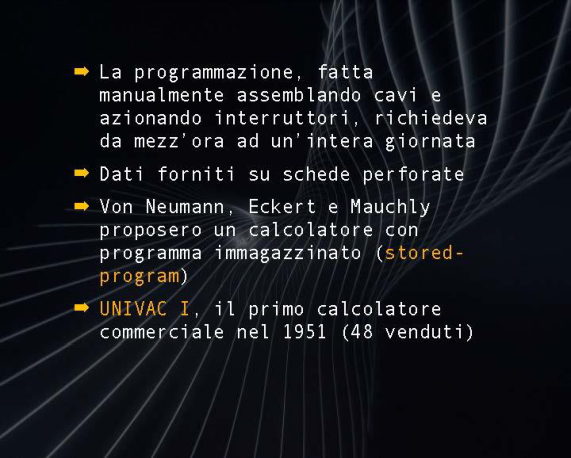
\includegraphics[width=0.6\linewidth]{images/Lez01_p01_fig_05.png}
    \caption{Slide 5}
    \label{fig:slide_5}
\end{figure}

La programmazione  di Enec (slide \ref{fig:slide_5}) veniva fatta manualmente assemblando cavi e azionando interruttori e richiedeva tipicamente da mezz'ora a un'intera giornata.
Notate la frase assemblando, la parola assemblatore deriva esattamente dalla funzione degli operatori che andavano fisicamente ad assemblare cavi, muovere interruttori, aggiungere schede e parti per riprogrammare questo calcolatore.
Quindi non vi era un programma immagazzinato su un supporto di massa, un disco, una memoria stato solido, un nastro o qualunque altro mezzo di archiviazione, ma il programma veniva scritto fisicamente ogni volta ricablando e riposizionando degli interruttori.
Ovviamente era una cosa esageratamente primitiva dal nostro punto di vista ma è importante osservare anche alcune delle ragioni storiche che determinano l'uso di certi terminologie, in particolare del termine assemblatore.
I dati in uscita venivano forniti su schede perforate che era un sistema di rappresentazione dell'informazione in uscita abbastanza semplice ma comunque già gestibile dagli utenti in maniera ragionevolmente semplice.

In quegli anni anche Von Neumann, Eckhart e Mauclky proposero un calcolatore con un programma immagazzinato, quello che in inglese si chiama store program.
In questo caso per cambiare il programma non è più necessario ricablare il sistema, bensì è possibile caricarlo in qualche modo da qualche altra forma di supporto.
Questo è il concetto generale di tutti i programmi che noi ogni giorno utilizziamo, nessuno di noi penserebbe mai di dover ricablare il proprio calcolatore per poter svolgere una nuova funzione.

Di lì a poco Univac 1 fu il primo calcolatore commerciale ed entrò in commercio nel 1951, ben 48 pezzi furono venduti.
Anche questa è una macchina oggettivamente molto ingombrante, molto grande.
Di lì a poco seguì anche l'IBM, che era un'azienda che si occupava di sistemi di stampa, archivi e ufficio, quindi avevano chiaramente un mercato diretto da aggredire.
Questi piccoli cenni storici vi li do anche perché è importante contestualizzare le evoluzioni.

\begin{figure}[ht]
    \centering
    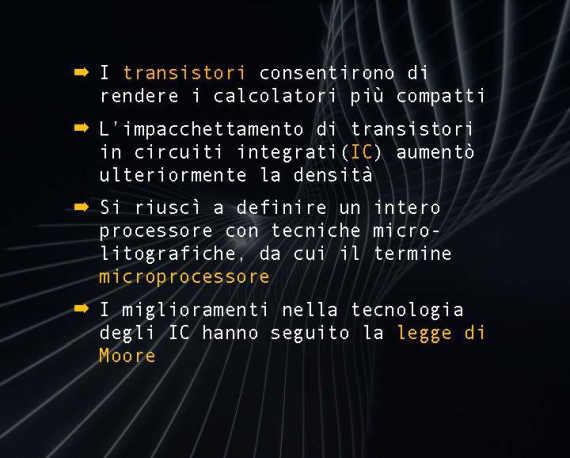
\includegraphics[width=0.6\linewidth]{images/Lez01_p01_fig_06.png}
    \caption{Slide 6}
    \label{fig:slide_6}
\end{figure}

I transistori (slide \ref{fig:slide_6}) a stato solido consentirono di rendere i calcolatori ben più compatti di quanto non erano mediante l'utilizzo di valvole a vuoto.
Col tempo si riuscirono a impacchettare transistori in circuiti integrati o integrated circuits in inglese e ciò aumentò ulteriormente la densità dei transistori per unità di superficie.
Questo è particolarmente importante, per poter fare cose più evolute e più potenti spesso è necessario avere più dispositivi.
Ricordate quello che vi ho detto in una delle precedenti slide, ENIAC aveva 18.000 valvole.
Se andate a stimare nell'ordine di qualche centimetro cubo il volume di una valvola fate presto a fare i conti di quanto è ingombrante il sistema.
Oggigiorno un transistore ha delle dimensioni fra i 20 e i 14 nanometri, come di dimensione del disegno.
Ovviamente è una struttura prevalentemente bidimensionale e quindi il volume reale dei dispositivi di commutazione è veramente esiguo, quello che vincola prevalentemente è la superficie e non tanto il volume in questo caso.

Col passare del tempo e dello sviluppo tecnologico si riuscì a definire un intero processore con tecniche microlitografiche da cui ha anche il termine di microprocessore, cioè si riuscirono a mettere tutti i transistori in un solo chip, cioè una lastrina di silicio, in modo tale da poter svolgere tutte le funzioni.
Il primo microprocessore propiamente detto fu sviluppato nel 1971 e fu utilizzato dalla Texas Instruments per una piccolissima calcolatrice, tipicamente quella con cui voi normalmente fate somme e sottrazioni o poco più.
Ovviamente doveva essere un sistema a bassissimo costo, doveva essere venduto in un oggetto veramente consumer, cioè di largo utilizzo e ovviamente non particolarmente dedicato.

Quindi i primi microprocessori furono veramente delle macchine minimaliste, spesso a 4 bit, sia quello della Texas Instruments, il TMS 1000, che di lì a pochissimi mesi il 4004 dell'Intel, che fu un antisignano di una lunghissima generazione di processori che di fatto determinano che questa azienda in buona parte domini una parte del mercato, non tutti i mercati, ma una parte dei mercati.

I miglioramenti della tecnologia dei circuiti integrati hanno seguito la cosiddetta legge di Moore.

Nel caso voi non abbiate già avuto occasione di leggere o sentirla nella definizione corretta, ve la do nella slide \ref{fig:slide_7}.

\begin{figure}[ht]
    \centering
    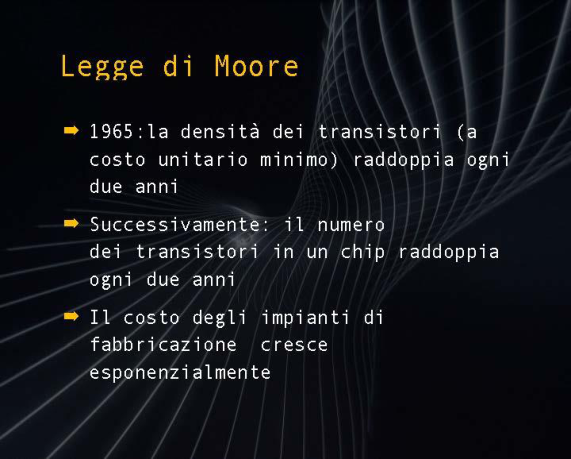
\includegraphics[width=0.6\linewidth]{images/Lez01_p02_fig_01.png}
    \caption{Slide 7}
    \label{fig:slide_7}
\end{figure}

La versione formulata nel 1965 da Gordon Moore, uno dei fondatori della Intel: \textit{"La densità dei transistori a costo unitario minimo raddoppia ogni due anni".}
%11:56
Questa osservazione fu fatta da una semplice osservazione sperimentale dell'andamento degli ultimi anni, da quando si era cominciato a integrare un numero di transistori crescente sullo stesso chip di silicio.
Quello che osservò Gordon Moore fu che era possibile ogni due anni raddoppiare il numero dei transistori mantenendo il minimo prezzo per transistore.
Da questa formulazione ne derivò una formulazione differente, quasi un corollario, che successivamente si disse che il numero dei transistori in un chip raddoppia ogni due anni.
Notate le due formulazioni sembrano identiche ma in realtà non lo sono.
Quello che è importante osservare non è che a prescindere da tutto il numero dei transistori raddoppi ogni anno, quello che succede è che è possibile realizzare transistori a costo minimo con un costo che permette l'aumento della densità di un fattore 2.
Sfortunatamente a questa crescita esponenziale del numero dei transistori per unità di superficie è anche derivato che il costo degli impianti di fabbricazione cresce esponenzialmente.
Quindi l'industria vive solo se è in grado di produrre sempre più transistori per mantenere lo stesso volume di mercato.
Ovviamente poi aggredisce anche nuovi mercati e questo fa sì che gli investimenti possono crescere e quindi gli sviluppi andare oltre.
Le ultime due righe ci dicono che sostanzialmente per molti anni voi avete pagato la stessa cifra per avere delle performance che in buona sostanza in prima approssimazione raddoppiavano.

I miglioramenti nei linguaggi di programmazione ad alto livello inoltre hanno reso sostanzialmente desueti i linguaggi assemblativi.
Questa è un'altra caratteristica importante dell'industria dei calcolatori.
Non c'è solo l'hardware che si è evoluto ma siamo passati da una situazione in cui programmavamo i computer, i calcolatori, mediante cablaggi di fili e interruttori meccanici operati da assemblatori, cioè da esseri umani, a linguaggi macchina in cui venivano immagazzinati degli 0 e degli 1 su qualche supporto di massa a una descrizione con linguaggi assemblativi che erano un po' più semplici, praticamente rappresentativi da lingua inglese, add, sub, move, load and store per questo richiamo la vostra attenzione al corso del primo livello architettura dei calcolatori e progettazione dei sistemi digitali in cui abbiamo già definito molte di queste istruzioni a livello assembler.
Con gli anni poi si sono sviluppati i linguaggi descrittivi, ad esempio il Fortran che è un linguaggio Formula Translation che permette di rappresentare più facilmente le equazioni, quindi risolvere problemi numerici, fino a linguaggi ad alto livello sempre più user-friendly, più vicini all'operatore.

L'utilizzo di linguaggi ad alto livello consente al programmatore di scrivere un numero di istruzioni maggiore al crescere del tempo.
Questo non sempre arriva senza una perdita di efficienza in termini di implementazione macchina, però le performance delle macchine, quindi dei processori, sono aumentate sempre più fino a molte volte a mascherare queste eventuali inefficienze.
Inoltre, con l'aumento dell'efficienza dell'hardware è anche migliorata la codifica dei compilatori che permettono di rendere ancora più efficiente la compilazione, quindi dal codice compilato a un codice assemblativo e dal codice assemblativo al codice oggetto.
La cosa interessante è che essendo diventati sempre più complicati i microprocessori è diventato sempre più difficile per l'umano scrivere un codice assembler che risulti più efficiente di quello scritto dalle macchine stesse, cioè dal compilatore.
Sebbene noi ogni tanto faremo richiamo comunque ai linguaggi assemblativi osserviamo che per problemi piuttosto grandi l'utilizzo dell'assemblatore sostanzialmente è venuto meno.
Vi possono ancora essere delle attività di nicchia in cui l'assemblatore è rilevante, per esempio la gestione dell'input-output con grande efficienza, alcune piccole architetture molto dedicate di tipo embedded, ma generalmente un programma d'uso generale non viene mai più scritto in linguaggio assemblativo.

\begin{figure}[ht]
    \centering
    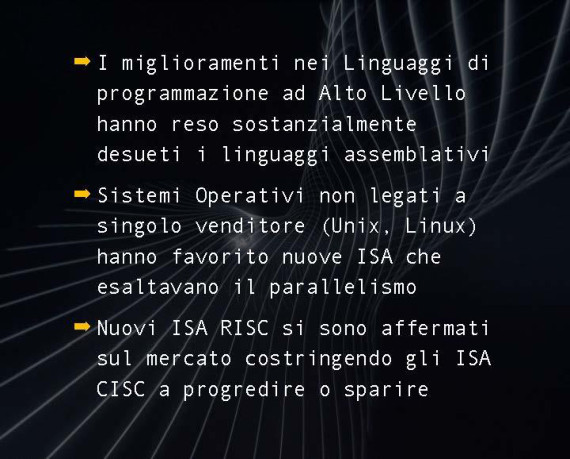
\includegraphics[width=0.6\linewidth]{images/Lez01_p02_fig_02.png}
    \caption{Slide 8}
    \label{fig:slide_8}
\end{figure}


Inoltre, negli anni oltre allo sviluppo di linguaggi di programmazione sempre più evoluti ad alto livello, in particolare negli anni 80 e primi anni 90 si affermarono dei sistemi operativi non più legati a un singolo venditore, unix prima e il suo clone Linux, che hanno favorito nuove architetture dei calcolatori, le instruction set architecture (ISA).
Noi useremo spesso l'acronimo pronunciandolo anche all'italiana ISA, sapendo che intendiamo l'insieme delle istruzioni che descrivono l'architettura. 
Anche per questo richiamo la vostra attenzione al corso della laurea di primo livello.
Queste architetture esaltavano ulteriormente il parallelismo, cosa che permetteva di aumentare le performance, in particolare il parallelismo a livello di istruzione delle nuove architetture RISC che si sono affermate sul mercato e queste affermandosi hanno accostretto le architetture CISC a provvedire oppure a sparire.

Negli anni della grande guerra fra CISC e RISC, tipicamente a cavallo della metà degli anni 90, molte architetture gloriose e anche veramente interessanti dal punto di vista architetturale sono sostanzialmente venute meno e si sono affermate, diciamo architetture CISC, e si sono affermate diverse architetture RISC.
Con il passare del tempo, quindi come abbiamo detto, queste architetture RISC hanno costretto i produttori di CISC o a evolvere oppure a scomparire.

\begin{figure}[ht]
    \centering
    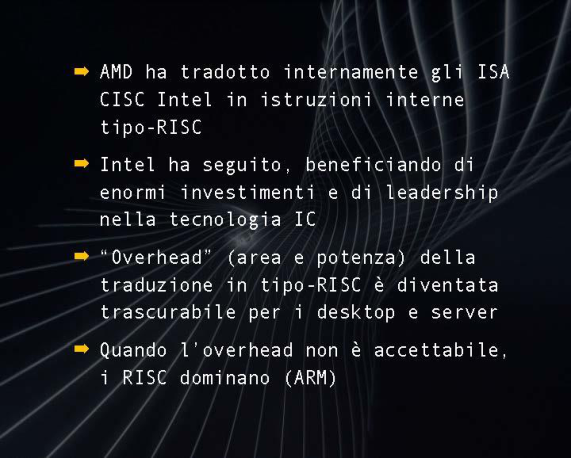
\includegraphics[width=0.6\linewidth]{images/Lez01_p02_fig_03.png}
    \caption{Slide 9}
    \label{fig:slide_9}
\end{figure}


Una delle architetture CISC dominanti, quella Intel, è stata adottata anche dalla AMD che ha inizialmente tradotto internamente le istruzioni dell'architettura CISC Intel in istruzione di tipo RISC, quindi utilizzando un sistema di decodifica di queste istruzioni, istruzioni che richiamandomi sempre ai corsi precedenti, avete già osservato, non essere particolarmente semplici da gestire perché hanno una lunghezza variabile, hanno strutture di prefissi, sostanzialmente molto poco gestibili, che vengono sostanzialmente inizialmente transcodificate in nuove istruzioni di tipo RISC ed eseguite internamente.
L'Intel ha capito immediatamente che questa era la via da seguire, quindi ha seguito beneficiando di enormi investimenti, essendo leader del mercato e della sua leadership nella tecnologia dei circuiti integrati.

Notate che sempre negli anni 90 la maggior parte dei produttori di nuove architetture di processore, di nuove instruction set architectures, avevano anche le loro attività di fonderia, cioè vi era uno sviluppo simultaneo sia dell'architettura hardware che della tecnologia per implementarla.
Questa era vero per AMD, era vero per Intel, era vero per MIPS, DEC, Digital Equipment che produceva Alfa, probabilmente per molti anni uno dei processori più performanti, delle famiglie di processori più performanti, ma con gli anni quello che è successo è che questa pletora di architetture RISC che comunque coprivano delle nicchie di mercato, anche spesso delle nicchie di alto livello, hanno cominciato a perdere terreno perché l'overhead, cioè il sovraccarico in termini di area e potenza della traduzione da instruction di tipo CISC a instruction di tipo RISC è diventata trascurabile per la maggior parte dell'architettura di desktop e dei servers.
Cosa significava?
Come vi ho detto all'inizio, per tradurre le instruction CISC originarie in architetture RISC era necessario realizzare un insieme di circuiti di codifica.
Però con le leggi di scaling, le leggi di Moore, la quantità di transistor necessaria per tradurre queste instruction rimaneva costante e quindi veniva a occupare un'area sempre decrescente sul chip fino al punto che è diventata sostanzialmente trascurabile nella maggior parte dei casi.

Considerate che un chip di un processore contiene prevalentemente delle memorie.
Vi chiamo anche la vostra attenzione alla generarchia di memorie.
Quindi questa piccola parte di transcodifica diventava sempre più piccola in termini di superficie e anche in termini di consumi di potenza.
Solo quando l'overhead non era accettabile i RISC hanno continuato a dominare il mercato.

\begin{figure}[ht]
    \centering
    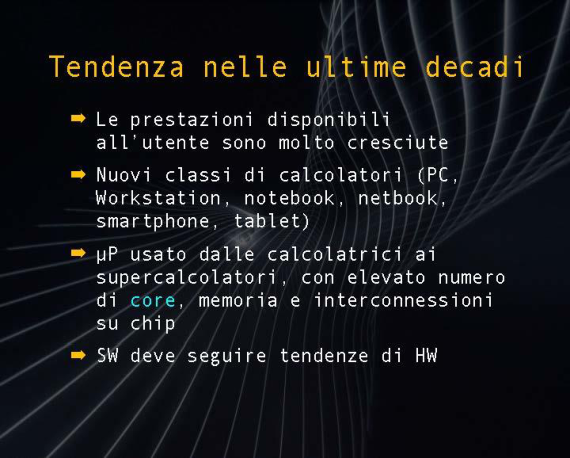
\includegraphics[width=0.6\linewidth]{images/Lez01_p02_fig_04.png}
    \caption{Slide 10}
    \label{fig:slide_10}
\end{figure}


Così abbiamo adesso una tendenza nelle ultime decadi, negli ultimi decine di anni.
Le prestazioni disponibili all'utente sono molto cresciute.
Di questo chiunque di noi se ne accorge semplicemente cambiando computer, cambiando portatile, cambiando cellulare, ma soprattutto ci consente di fare delle cose che non avremmo mai pensato di fare pochi anni orsono.
Nuove classi di calcolatori partendo dai grandi computer corporate, i cosiddetti mainframe, in termini di PC, war stations, notebook, netbook, smartphone e tablets, hanno avuto avvento nel mercato.
Dal punto di vista del motore di calcolo, il microprocessore è ormai usato partendo dalla semplice calcolatrice da tavolo ai supercalcolatori.
Con supercalcolatori con un elevato numero di core, di memorie e di interconnessioni, tutte oramai su chip.
Quindi si cerca un livello sempre più elevato di integrazione per portare quanto più possibile gli elementi all'interno dello stesso chip.
Ci accorgeremo nel corso del corso che questo è un beneficio sia in termini performance che di costi, ma soprattutto di consumi di potenza che sono dei problemi più critici oramai nell'industria.

La cosa più difficile è che il software deve seguire le tendenze dell'hardware.
Non è sufficiente, come vi ho detto, semplicemente scalare il numero di transistori e mettere sempre più transistor nello stesso chip.
È anche necessario evolvere i linguaggi di programmazione in maniera tale che questi riescano a ottenere il meglio dall'architettura hardware.
Vi ho detto ad esempio che i linguaggi ad alto livello ormai fanno sì di poter sfruttare meglio i livelli di parallelismo, ad esempio, delle istruzioni.
Questo è un cenno ma sarà una parte importante del corso.
%23:46

\begin{figure}[ht]
    \centering
    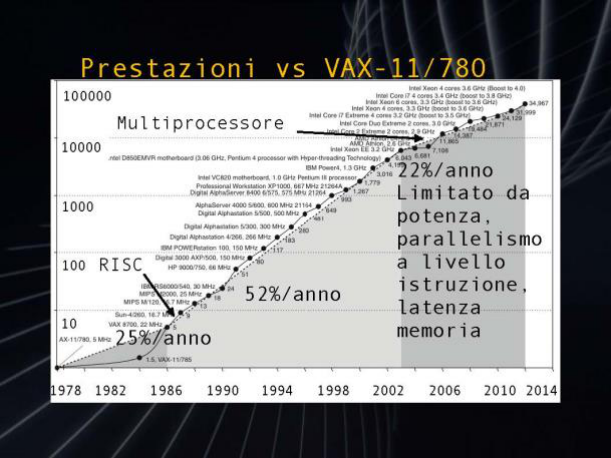
\includegraphics[width=0.8\linewidth]{images/Lez01_p02_fig_05.png}
    \caption{Slide 11}
    \label{fig:slide_11}
\end{figure}


Consideriamo quindi un esempio tipico.

Questa è una tabella molto interessante perché mostra, misurate secondo un benchmark, cioè uno standard di misurazione internazionale, lo SPEC, l'evoluzione delle performance a partire dal 1978, calcolate rispetto a un mini computer della digital equipment, il VAX 11/780, che è una macchina di riferimento per l'industria, e si vede come le performance o prestazioni sono aumentate negli anni fino ad arrivare a circa 35.000 volte quello che si otteneva nel 1978, quindi diciamo nell'arco di 36 anni il livello delle performance è aumentato di 35.000 volte.
Una cosa importante su questo grafico sono le tendenze.
Nei primi anni in cui i calcolatori non erano basati su un microprocessore singolo, ma su un insieme di chip distinti, assemblati su una scheda, i tassi di crescita erano nell'ordine del 25\%.

Nella metà degli anni 80 presero l'avvento i vari RISC, si scatenò una cosiddetta battaglia dei RISC vs CISC che comportò un aumento del 52\% tendenziale anno su anno in cui non solo vi era la legge di Moore che consentiva l'aumento del numero dei transistori per unità di superficie, ma anche miglioramenti architetturali a livello di istruzione, cioè il pipeline prima, l'esecuzione fuori ordine, le cache, l'esecuzione speculativa di cui vi è stato raccontato nei corsi del primo livello, hanno fatto sì che la tendenza fosse nell'ordine del 52%.
E' impressionante come questa curva su questo grafico semilogaritmico abbia praticamente questo andamento costante.

A un certo punto nei primi anni 2000, attorno a 2003 in particolare, c'è stato il cosiddetto power wall, cioè il muro della potenza, non era più possibile aumentare le performance aumentando il numero di transistor e l'aumento della potenza, ma era necessario passare alla cosiddetta architettura a multiprocessore, a multicore anche sullo stesso chip.
Questa era l'unica soluzione da poter seguire, ma ha comportato chiaramente un aumento limitato delle performance a solo il 22\% anno su anno.
Le limitazioni erano legate al fatto che non si poteva aumentare la dissipazione della potenza, che il livello di parallelismo e livello di istruzione era non più espandibile ulteriormente e anche il collo di bottiglia degli accessi alla memoria, sia in termini di banda che in termini di latenza, di cui parleremo fra breve.


\begin{figure}[ht]
    \centering
    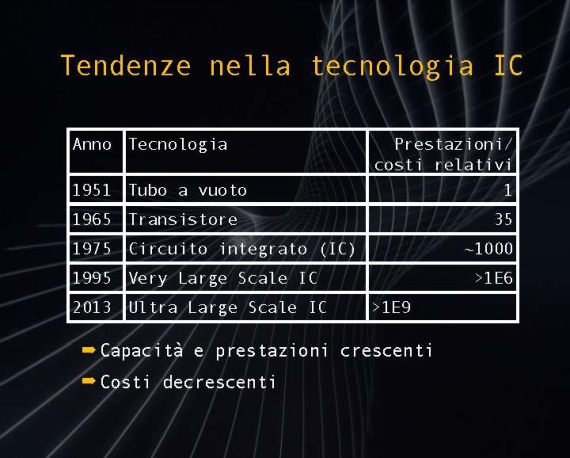
\includegraphics[width=0.6\linewidth]{images/Lez01_p02_fig_06.png}
    \caption{Slide 12}
    \label{fig:slide_12}
\end{figure}

Vi faccio vedere qui in questa tabella le tendenze nella tecnologia dei circuiti integrati.
L'elemento di calcolo nel 1951, quando entrò in commercio il primo Univac, era il tubo a vuoto e consideriamo questo come elemento unitario in termini di rapporti prestazioni costi.
Nel 65 furono adottati i transistori e si ebbe un vantaggio, come vedete, già nell'ordine del 35.
Nel 75 erano di fatto standardi circuiti integrati a diversi livelli di integrazione, tipicamente con rapporti prestazioni costi rispetto al tubo a vuoto dell'unico Univac 1 di circa mille.
Nel 95 il cosiddetto pre-large scale integration consentiva ormai di integrare nell'ordine di alcuni milioni di transistori sullo stesso chip.
Nel 2013 si integrano alcuni miliardi di transistori sullo stesso chip, la cosiddetta ultra large scale integration.

Credo che non troveremmo ulteriori modi per definire la crescita di numero di transistori negli anni, ma chiaramente è impressionante come le prestazioni costi sono andate quasi di pari passo con il numero degli elementi, cioè aumentano le prestazioni a parità di costo e quindi è stato possibile mettere sempre più elementi nello stesso chip.
Quindi osserviamo capacità e prestazioni crescenti e costi decrescenti.


\begin{figure}[ht]
    \centering
    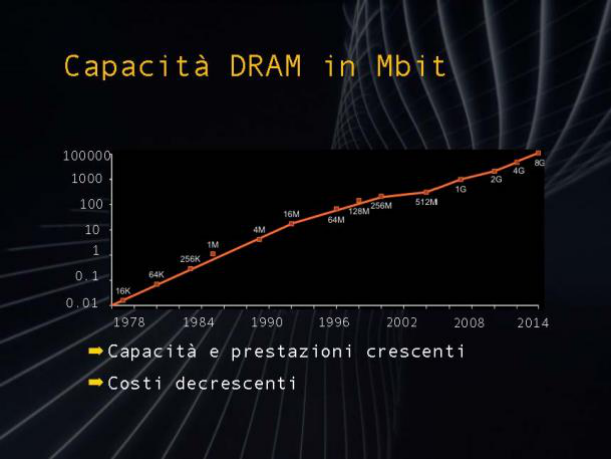
\includegraphics[width=0.8\linewidth]{images/Lez01_p03_fig_01.png}
    \caption{Slide 13}
    \label{fig:slide_13}
\end{figure}

In questo caso vi faccio vedere un grafico molto significativo (slide \ref{fig:slide_13}), quello dell'andamento della capacità delle memorie dinamiche DRAM misurate in megabit. Si passa sempre dal 1978 con 16 kilobit fino a 8 gigabit nel nel 2014.
Notate anche questo andamento quasi costante in scala semi logaritmica e un certo livello di saturazione anche in questo caso attorno al 2003, l'anno in cui anche i microprocessori hanno smesso di correre al 52\% di crescita anno su anno.


\begin{figure}[ht]
    \centering
    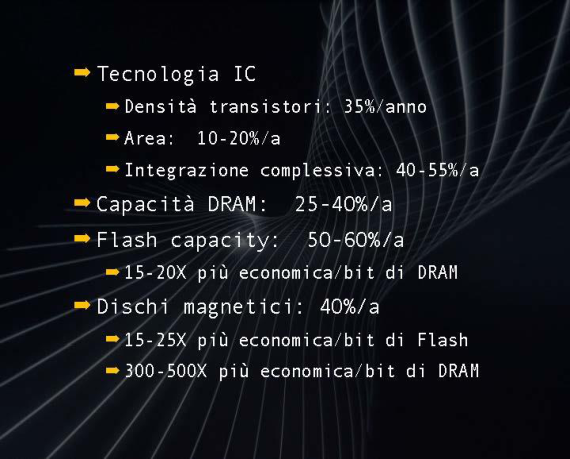
\includegraphics[width=0.8\linewidth]{images/Lez01_p03_fig_02.png}
    \caption{Slide 14}
    \label{fig:slide_14}
\end{figure}

Vediamo alcune caratteristiche salienti degli scaling delle tecnologie dei circuiti integrati slide \ref{fig:slide_14}.

Osserviamo che la densità dei transistori è cresciuta sostanzialmente al 35\% su anno, molto prossima alla tradizione della legge di Moore che diceva raddoppio ogni 2 anni, cioè radice di 2 all'anno, quindi molto vicina al 35\%.
L'utilizzo dell'area è cresciuto di circa il 10-20\% anno su anno determinando quindi un'integrazione complessiva, cioè il numero di transistori complessivi per chip nell'ordine del 40-55\%.
Sono aumentate le aree e quindi la legge di Moore nella sua formulazione originaria è rimasta verificata.
La capacità delle DRAM è cresciuta ad esempio nell'ordine del 25-40\%, come avete visto c'è stato un livellamento negli ultimi anni, scendendo verso il 25.
Le capacità delle memorie a stato solido permanenti, le flash tra il 50 e il 60\%, quindi quelle che crescono più velocemente e sono diventate ormai fra il 15 e il 20 volte più economiche per bit delle DRAM, infatti le trovate in qualunque dispositivo in grande abbondanza a costi molto modesti, tipicamente nell'ordine del mezzo dollaro per megabyte, attualmente.
I dischi magnetici sono cresciuti anch'essi con una regola di scaling molto prossima a quella dei circuiti integrati intorno al 40\% anno su anno e risultano ancora oggi ben più economici delle flash per un rapporto circa di 15-20 volte rispetto alle flash e addirittura di 300-500 volte più economiche per bit delle DRAM.
Questo è uno dei motivi per cui si usano ancora delle gerarchie di memorie e memorie virtuali di cui richiamo la vostra attenzione ai contenuti del corso di laurea del primo livello.


\begin{figure}[ht]
    \centering
    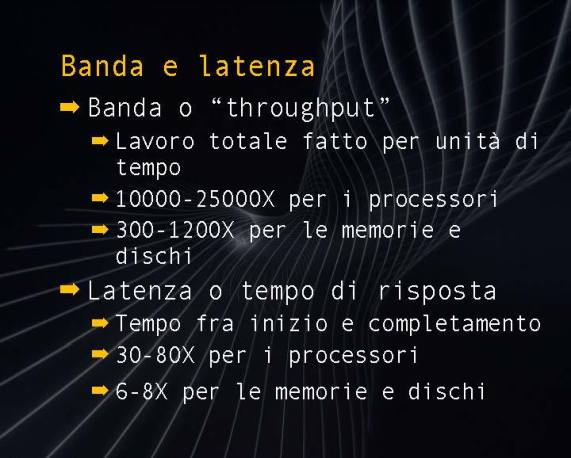
\includegraphics[width=0.6\linewidth]{images/Lez01_p03_fig_03.png}
    \caption{Slide 15}
    \label{fig:slide_15}
\end{figure}


\section{Banda e latenza}

Definiamo il concetto di banda e latenza (slide \ref{fig:slide_15}).

La banda o throughput in inglese, cioè la quantità di cose che passano attraverso, questa è esattamente la traduzione di throughput dall'inglese all'italiano.

Può anche essere definito come il lavoro totale fatto per unità di tempo.

I processori questo aumento è stato fra 10.000 e 25.000 volte, fra 300 e 1.200 per le memorie DRAM e i dischi, 

La latenza o tempo di risposta è invece un altro parametro importante ed è il tempo fra inizio e completamento di una particolare operazione.
Quindi le due cose non sono necessariamente correlate, uno può avere un sistema con un'elevatissima banda ma una latenza poco soddisfacente, o al contrario uno può avere latenze molto basse ma bande più limitate.

È chiaro che in molte situazioni è importante avere un grande trasferimento di dati, immaginate ad un disco magnetico, ma la latenza è legata alla rivoluzione del disco, tipicamente il mezzogiro come valore medio e alla traslazione delle testine lungo l'asse radiale, il raggio del disco.
Questo ovviamente termina delle latenze di alcuni millisecondi ma poi il throughput è in ordine del centinaio abbondante di megabyte per secondo.
Quindi in alcune situazioni questa latenza è accettabile soprattutto se non la si usa come memoria virtuale.
Chiaramente i vantaggi dell'utilizzo di una memoria flash come memoria virtuale sono molto elevati ma vi richiamo anche alcune criticità nell'uso delle flash come memoria virtuale.

I tempi di risposta sono aumentati, le latenze sono diminuite di un fattore 30-80 per i microprocessori ma per le memorie e per i rischi queste latenze sono diminuite molto meno.

Quindi come vi ho detto le performance complessive di un calcolatore non sono determinate solo da uno di questi parametri ma da una combinazione di parametri in particolare legati al tipo di applicazione che si deve fare.

\begin{figure}[ht]
    \centering
    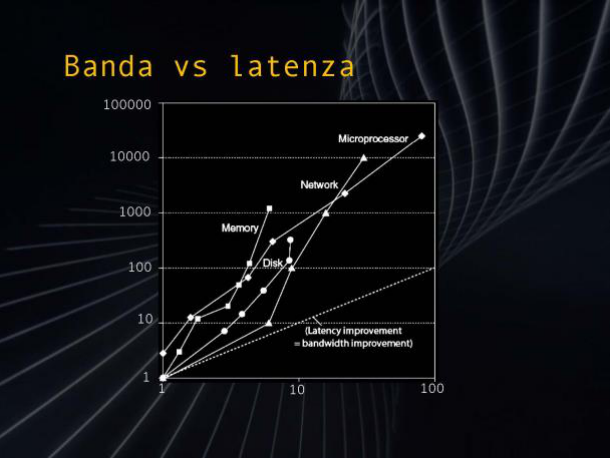
\includegraphics[width=0.8\linewidth]{images/Lez01_p03_fig_04.png}
    \caption{Slide 16}
    \label{fig:slide_16}
\end{figure}

Guardiamo un altro grafico (slide \ref{fig:slide_16}) che è esemplificativo, qui graficiamo sull'asse delle asciisse la latenza e sull'asse delle ordinate la banda.
Vedete come i microprocessori, le reti di comunicazione, i dischi e le memorie hanno avuto degli andamenti differenti.
Idealmente avremmo dovuto avere che la latenza migliorava esattamente come la banda, sfortunatamente la latenza non è migliorata come la banda, è aumentata di più la banda ma la latenza ritarda a migliorare.

Questo è un problema abbastanza critico perché pur aumentando alcune delle performance, la capacità di esecuzione, la quantità di dati che passa per unità di tempo verso l'interfaccia di memoria, in realtà non è che aumentiamo il throughput in modo proporzionale perché spesso siamo legati alla latenza che non è cresciuta.

\section{Tendenze architetturali}

\begin{figure}[ht]
    \centering
    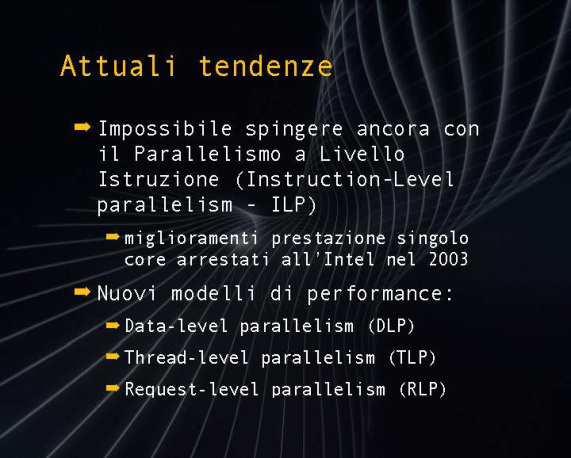
\includegraphics[width=0.8\linewidth]{images/Lez01_p03_fig_05.png}
    \caption{Slide 17}
    \label{fig:slide_17}
\end{figure}

Guardiamo alcune delle attuali tendenze architetturali. (slide \ref{fig:slide_17})

Osserviamo che è impossibile spingere ancora con il parallelismo a livello di istruzione, il cosiddetto instruction level parallelism o ILP e che i miglioramenti della prestazione di un singolo core si sono arrestati con l'Intel nel 2003.
Questo è significativo perché mentre fino alla fine degli anni 90 c'erano delle architetture puramente RISC a dominare il mercato, nei primi anni 2000 vi è stata un po' una battaglia fra AMD e Intel nelle loro implementazioni della stessa architettura, come vi ho detto le architetture che hanno un decoder e internamente sono sostanzialmente di RISC, non più dei CISC, ma ricevono ancora delle istruzioni di CISC, dalla 2003-2004 praticamente le architetture Intel dominano in termini di performance e il miglioramento delle performance sono non più legate al miglioramento del singolo processore ma all'utilizzo di più processori.

Quindi sono necessari dei nuovi modelli di performance o di prestazione quella a livello del parallelismo dei dati, cioè il data level parallelism, di cui parleremo ampiamente e quello a livello di thread level parallelism, cioè a livello di trama e a livello di richiesta di servizio, quindi useremo sempre i termini inglesi, perché sennò quelli italiani sfortunatamente poi non li capisce nessuno fuori dal contesto.

\section{L'era post PC}

\begin{figure}[ht]
    \centering
    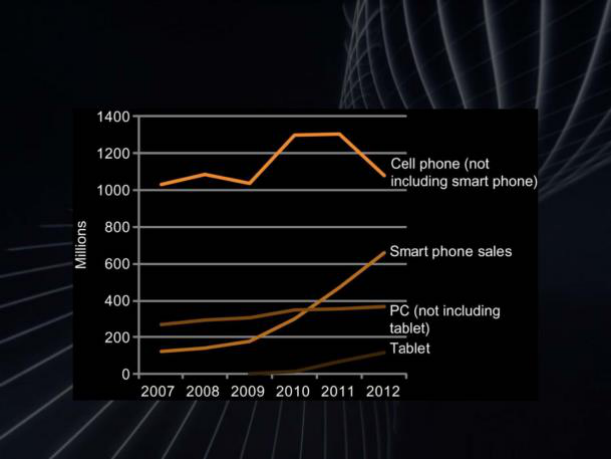
\includegraphics[width=0.8\linewidth]{images/Lez01_p04_fig_01.png}
    \caption{Slide 18}
    \label{fig:slide_18}
\end{figure}


Per era post PC  intendiamo quella fase di sviluppo dell'industria dei calcolatori in cui non c'è più l'oggetto da tavola convenzionale in cui uno ha un monitor, uno schermo, una tastiera, eventualmente un mouse come sistema di interfaccia che è legato alla struttura, non c'è neanche un notebook, cioè l'equivalente scalato in una dimensione più bassa, ma in cui il mezzo di interfaccia è sempre la tastiera e se non più un mouse ma al limite un trackball, un puntatore, un tappetito, un tappetino con cui si sposta, ma sostanzialmente un ausilio alla tastiera e in cui la forma di rappresentazione, l'uscita è prevalentemente un monitor, ma in tutta quella generazione di dispositivi in cui cambia il modo di interfacciarsi con il calcolatore.

Prima di andare a vedere cosa intendiamo, andiamo a vedere anche l'andamento nel mercato negli ultimi anni (slide \ref{fig:slide_18}).
Notate come il mercato dei PC, dei personal computers, escludendo le strutture tipo tablet, è cresciuto, ma è cresciuto a un tasso sensibilmente più basso di quello dei cosiddetti smartphone, dei telefoni intelligenti.
Qui stiamo parlando di numeri enormi, cioè di 700 milioni nel 2013, allo stesso tempo i telefoni cellulari che erano cresciuti notevolmente negli anni 80, 90 e i primi anni 2000, diciamo i telefonini con cui si telefonava, si mandava un massaggio di testo, hanno cominciato a decrescere nei numeri e con grande piacere dell'industria perché il prezzo di vendita dei cosiddetti smartphone è nettamente superiore a quelli dei telefoni convenzionali che si acquistano per poche decine di euro e sulla quale non fa soldi quasi più nessuno.
Notate anche come a partire dal 2010 hanno preso avvento anche i cosiddetti tablet che stanno crescendo con dei tassi di crescita non esattamente uguali a quelli dei telefoni, dei smartphone, ma quasi simili.


\begin{figure}[ht]
    \centering
    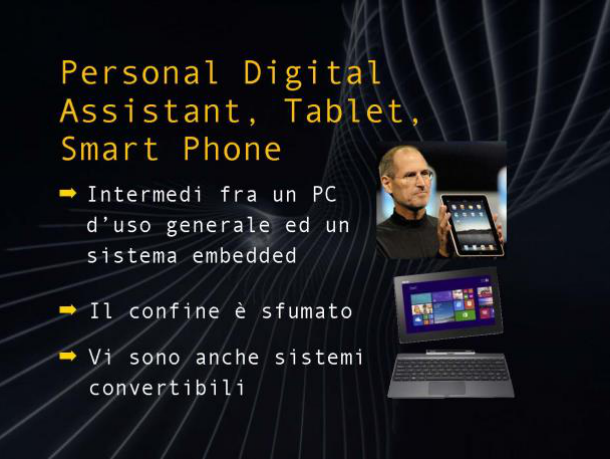
\includegraphics[width=0.6\linewidth]{images/Lez01_p04_fig_02.png}
    \caption{Slide 19}
    \label{fig:slide_19}
\end{figure}


Nella categoria che andiamo a considerare (slide \ref{fig:slide_19}),  quindi ci sono i cosiddetti personal digital assistance, tablets, smartphones, chiamati a volte anche personal mobile devices, spesso nel corso e anche nei libri di testo verranno chiamati PMD.
Sono intermedi tra un PC d'uso del generale e un sistema embedded introdotti da questo signore Steve Jobs con la sua azienda la Apple che compiangiamo tutti per la scomparsa prematura.
Il confine tra un computer d'uso embedded e un computer d'uso generale è molto sfumato e per questo un tablet, un smartphone hanno entrambe le funzioni o parte di entrambe le funzioni.
Vi sono anche dei sistemi convertibili, cioè praticamente una tastiera convenzionale che può essere connessa al resto del tablet, quindi diciamo o un tablet standard come questo iPad che può essere utilizzato per esempio con una tastiera esterna Bluetooth, quindi diciamo la distinzione fra un computer d'uso generale e un tablet è veramente sfumata.


\begin{figure}[ht]
    \centering
    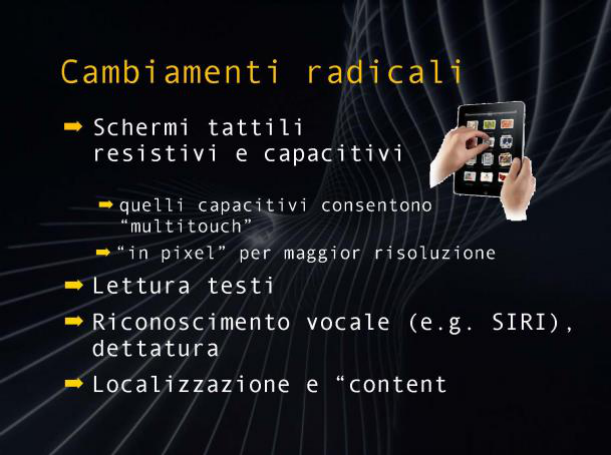
\includegraphics[width=0.6\linewidth]{images/Lez01_p04_fig_03.png}
    \caption{Slide 20}
    \label{fig:slide_20}
\end{figure}

%39:59

Vi sono però dei cambiamenti radicali (slide \ref{fig:slide_20}), ormai nessuno più è costretto a usare una tastiera o un mouse, si va, si clicca, si allarga, si gira, si ruota con le dita e l'interfaccia vera e propria sono diventate le nostre dita che agiscono su schermi tattili o touch screens di natura resistiva o capacitiva.
Dopo una certa lotta iniziale quelli capacitivi sembrano dominarie perché consentono le cosiddette funzioni multitouch a 2, 3 o addirittura 4 dita contemporanea per fare delle funzioni più importanti.
Tipicamente su uno di questi oggetti volete ruotare un'immagine, la girate con la tua dita e quella ruota.
Non immaginate la quantità di codice bisogna scrivere dietro per fare questo.
In alcuni casi vi sono anche dei sensori in pixel, cioè si implementano dei capacitori all'interno del singolo pixel del display a cristalli liquidi per avere una maggiore risoluzione, questo non viene senza costi.
L'interfaccia d'uscita consente ad esempio di leggere automaticamente i testi, quindi non doverli vedere a video, molto utile per esempio in automobili, il riconoscimento vocale è anche molto utile per avere le mani libere, il cosiddetto Siri, ad esempio della Apple e analoghi sistemi, con la possibilità di dettare direttamente e non usare più a questo punto neanche le mani per comunicare con la macchina.
Inoltre questi sistemi hanno dei sistemi di localizzazione, di cosiddetto content awareness, cioè capiscono quello che devono fare quasi da soli.


\begin{figure}[ht]
    \centering
    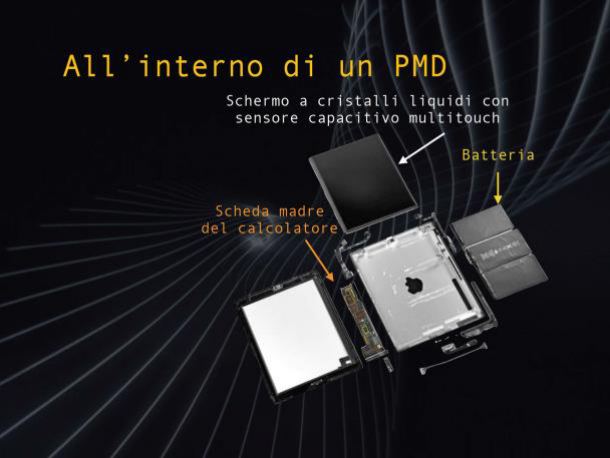
\includegraphics[width=0.8\linewidth]{images/Lez01_p04_fig_04.png}
    \caption{Slide 21}
    \label{fig:slide_21}
\end{figure}

Vediamo cosa c'è all'interno di un person mobile device, questo è un iPad 2 (slide \ref{fig:slide_21}).

Notate lo schermo capacitivo a cristalli liquidi, la batteria, la scheda madre vera e propria, cioè quello che chiameremo il calcolatore in un termine storico.

\begin{figure}[ht]
    \centering
    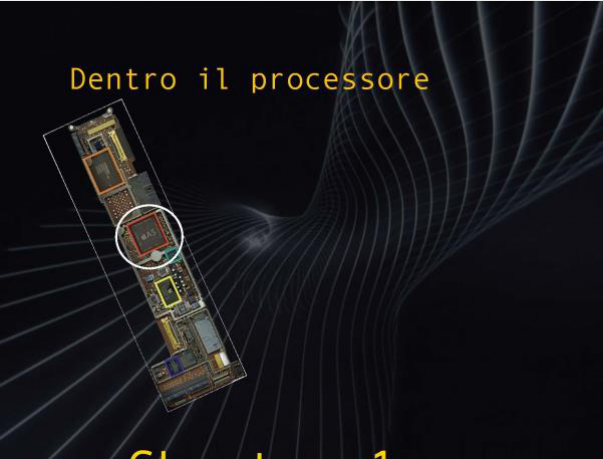
\includegraphics[width=0.8\linewidth]{images/Lez01_p04_fig_05.png}
    \caption{Slide 22}
    \label{fig:slide_22}
\end{figure}


Vi faccio uno zoom (slide \ref{fig:slide_22}), vedete che è fatto da un microprocessore, in questo caso un Apple A5, dentro il processore osserviamo che le unità di calcolo sono due core arm, in questa zona qui uno e due, un bel po' di cache onboard, quattro unità di calcolo grafico, come vedete la parte grafica occupa più spazio del vero e proprio calcolo e una marea di blocchi logici dedicati, proprietari, le interfacce sdram, l'interfaccia d'ingresso uscita e così via.

\begin{figure}[ht]
    \centering
    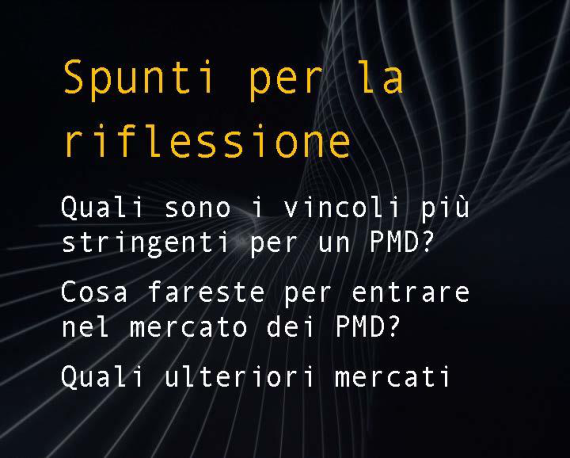
\includegraphics[width=0.8\linewidth]{images/Lez01_p04_fig_06.png}
    \caption{Slide 23}
    \label{fig:slide_23}
\end{figure}

Vi do adesso come sarà prassi alcuni spunti per la riflessione e vi invito a riflettere quali siano i vincoli più stringenti per un person mobile.
Vi invito anche a riflettere cosa fareste voi per entrare nel mercato dei person mobile device, se foste un'azienda, un imprenditore e infine vi invito a riflettere su quali ulteriori mercati prevedete per l'industria dei calcolatori.
In quest'ultima domanda però, ve la faccio, ma voi non date la risposta a nessuno e se lo sapete, meglio che ve lo tenete per voi.
Con questo vi saluto e vi rimando alla prossima lezione.


